\chapter{
Heuristics for System-Level Power Supply Design 
}
%system level

%Intuition for Wireless Sensor Power Supply Design
%Navigating design space
%Guidelines
%Entanglements
% more active titles
\label{chap:intuition}

%There is a rift between industry and research in the way that indoor wireless sensors are powered. Industry has largely eschewed energy harvesting methods, opting instead for the reliability offered by high-density non-rechargeable batteries. 
%Conversely, energy-harvesting is extremely popular for research systems, which have largely abandoned the use of non-rechargeable cells in the pursuit of building systems with indefinite lifetimes. 
%Given this disparity, it is obvious that there is a lack of clarity regarding how wireless sensors should be powered to enable various applications. 
Wireless power supplies are the result of a multi-dimensional design space exploration.
While certain design decisions are straightforward, like the choice to use a certain type of harvester to suit an application environment, some design points are more difficult to determine. 
Harvesting and storage technologies are often difficult to directly compare, and it is sometimes difficult to determine the sizing of these elements in order to satisfy the constraints of an application. 
Many times, the type and size of harvesters, batteries, or capacitors are chosen arbitrarily~\cite{hamiltoniot,lee2013modular,juang2002energy}, or are chosen to make the design minimally feasible~\cite{yervaGrafting12,debruin2013monjolo,hesterFlicker17,afanasov2020battery}.

The goal of this chapter is to provide high-level guidance for navigating the design space of wireless sensor power supplies. 
We formalize the the application requirements that were discussed in 
\cref{sec:background:background_reqs}.
Using these requirements, this chapter provides guidance to designers for when energy harvesting is a beneficial technique for energy income instead of, or in addition to, a non-rechargeable storage, how prospective income and workloads drive component types and sizing, and if energy-harvesting is utilized, what techniques are required to ensure a minimum useful operation or what is required to capture sufficient energy to maximize system availability. 
To limit scope of this chapter among those following to a manageable size we choose to focus exclusively on indoor photovoltaic energy harvesting.
%This is because in the conditions of the majority of human-occupied indoor locations, photovoltaic harvesting offers an order of magnitude more energy than other methods.
%Despite this focus, similar explorations can be made with other harvesting methods.
Occupied indoor environments are the focus of a significant
amount of
prior work, 
and for good reason: most
applications aim to improve the lives of people and are necessarily present
in the spaces they occupy~\cite{hesterTimely17,hesterFlicker17,colinReconfigurable18,campbellEnergy14} \hl{TODO better cites}.
%Even the example applications of intermittent, energy harvesting systems are nearly all centered around monitoring
%indoor and human-centric phenomena
Indoor environments are lit by both natural and artificial light, 
and may occasionally get direct or indirect sunlight. 
Under these conditions, photovoltaic harvesting still offers an order of magnitude more energy than other methods.
However, indoor environments still present a significantly more challenging and low power design space compared to the outdoor ones. 
The decision to focus on indoor photovoltaic harvesting does not mean that the conclusions drawn are not applicable to other
environments and harvesting methods, however design details may differ. 

\section{Energy Income}
\label{sec:intuition:energy_income}
A wireless sensor must source energy from somewhere. 
Energy-harvesting has the potential to supply energy indefinitely. However, harvested energy is often unreliable and unpredictable, and instantaneous power delivery is limited. 
Conversely, primary-only systems have a limited amount of energy, but can use that energy at any rate they please, within the power limits of the battery. 
Because of these differences, it can be difficult to directly compare their performance and determine at what scale and in which conditions harvesting, energy preallocation, or a hybrid of the two, is the preferable power source strategy for any given application.
This section begins with a description of constraints for properly sizing components to ensure a sufficient lifetime and energy income. 
Next, it provides a method of comparison of energy capture potential between harvesting and preallocation methods.
The constraints and relations defined and explored in the following section can be used to estimate proper harvester and battery selection to achieve application requirements.

\subsection{Sizing}
\label{sec:intuition:energy_income_sizing}
Regardless of how a sensor is powered, it must receive sufficient energy at the right times to continuously and reliably operate.
Assuming that the average power required to drive an application is known at design time, it is relatively straightforward to determine the correct size of a battery to achieve an expected lifetime, or a photovoltaic panel to achieve an average power income.
%The improvement in energy density of batteries and the efficiency of energy harvesting sources has not improved at the same rate as the energy efficiency of CMOS and low power radio technology.
%Barring any transformative improvements in energy storage, energy income is primarily dependent on the volume or area available for a battery or harvester, respectively. 
Usually battery capacity is expressed as accumulated charge in terms of \ssi{\milli\Ah}.
If the nominal voltage of the battery is known, it can be used to estimate lifetime given a battery's capacity and intended workload.

\begin{equation} \label{eqn:intuition:energy_battery_estimation}
   E_b = U C
\end{equation}
\begin{equation} \label{eqn:intuition:power_battery_estimation}
   \bar{P_b} = \frac{U C}{T} 
\end{equation}
%\begin{equation}
%   T \approx \frac{U*C}{P_{w}}
%\end{equation}

\noindent 
\Cref{eqn:intuition:energy_battery_estimation} describes the energy contained in a battery of capacity $C$ and a nominal voltage $U$. 
Assuming a desired lifetime $T$, \cref{eqn:intuition:power_battery_estimation} describes the maximum achievable average power supplied by such a battery. 
Likewise, the average power provided by a photovoltaic of area $A$ is described by \cref{eqn:intuition:p_power}. 

\begin{equation} \label{eqn:intuition:p_power}
\bar{P_h} = \eta \bar{E_e} A 
\end{equation}

\noindent 
Where 
$\eta$ denotes the efficiency of the photovoltaic, and is often between 18 and 20\%. 
The average energetic spectral irradiance, $\bar{E_e}$, is generally between 10 and 100\ssi{\micro\watt\per\centi\meter\squared} for photovoltaics in indoor conditions~\cite{yervaGrafting12,gorlatova2013networking}. 
Given an average workload power ($\bar{P_w}$) and a desired lifetime $T$, 
\cref{eqn:intuition:battery_capacity,eqn:intuition:panel_size}
describe the necessary battery capacity and solar cell size.

\begin{equation} \label{eqn:intuition:battery_capacity}
    C \geq \frac{\bar{P_w} T}{U}
\end{equation}
\begin{equation} \label{eqn:intuition:panel_size}
    A \geq \frac{\eta \bar{E_e}}{\bar{P_w}}
\end{equation}

For some applications, it is obvious when utilizing energy harvesting is a better design choice over a battery. 
Such is the case with Zebranet collars~\cite{juang2002energy}. Powering the collar would require a large and heavy battery, beyond the weight constraints of application, and would only power the system for 5 days, far below the lifetime goal of a year or more of operation.
In other cases, it is much more difficult to determine which method is appropriate.
This is especially apparent in environments where available harvestable energy is limited, like indoor environments. 


\subsection{Harvesting can Provide More Energy than Preallocation}
\label{sec:intuition:energy_income_pvh}
When potential harvestable energy is limited, it is difficult to determine whether energy preallocation or harvesting is the most suitable technique.
It is very difficult to directly compare these methods, as the power and energy supplied by either option is dependent on many factors, including the availability, variance, and magnitude of available harvestable energy, the size of the battery or harvester, and the expected sensor workload. 
%The most important metrics for consideration are the power and energy supplied by battery preallocation or energy harvesting.
%Energy income defines both the lifetime of a sensor, as well as a maximum supportable power available for a workload.
Prior work has attempted to approach a comparison of non-rechargeable energy storage and energy harvesting by comparing the expected average power supplied by either option. 
They simplify the problem by considering a theoretical cubic sensor of volume $V = L^3$, 
with the assumption that the entire cubic sensor volume is dominated by a lithium primary battery, or the entire area of one $A = L^2$ face is dominated by a photovoltaic panel~\cite{yervaGrafting12}.
The authors compare the power provided by the battery cube, with that of the photovoltaic square, over the shelf-life of the battery. 
%concluding that as sensors continue to reduce in size, they will derive more benefit from harvesting over battery preallocation. 

For this analysis, \cref{eqn:intuition:energy_battery_estimation} is not as useful for direct comparisons. 
%for comparing battery energy capacity with photovoltaic energy capture.
A more appropriate method utilizes volumetric energy density.
Battery energy capacity ($E_b$) can be estimated based on the volume of the battery ($V$) and its volumetric energy density ($\rho$).
While $\rho$ varies depending on the specific battery chemistry, size, and packaging, lithium primary batteries usually provide on the order of 800\ssi[per-mode=symbol]{\milli\Wh\per\cm\cubed}~\cite{tuna2016energy}. The maximum average power ($\bar{P_b}$) provided by the battery can be calculated with a desired lifetime ($T$). 

\begin{equation} \label{eqn:intuition:b_energy}
E_b = \rho V 
\end{equation}
\begin{equation} \label{eqn:intuition:b_power}
\bar{P_b} = \frac{\rho V}{T}
\end{equation}
%The volume of a sensor occupying a rectangular prism of dimensions $L$ length, $W$ width, and $H$ height is given by the following equation.
%
%\begin{equation}
%    V = L * W * H
%\end{equation}
%
%\noindent For an energy harvesting sensor, the side with the largest surface area represents the area available for harvesting with a photovoltaic. This area is represented by the following equation.
%
%\begin{equation}
%   A = L * W 
%\end{equation}
%
%Assuming that an application's power requirements are known before design, the the proper sizing of a battery and photovoltaic can be determined. 
%The energy and power stored in a battery of volume $V$ are described by the following relations:
%
%
%\noindent Where the energy density of the battery is $\rho$ 
%and $T$ is the lifetime of the battery.

\placefigure{fig:intuition:eh_worth_it}

\noindent When considering \cref{eqn:intuition:b_energy,eqn:intuition:b_power}, the authors use a more conservative 653\ssi[per-mode=symbol]{\milli\Wh\per\cm\cubed} for $\rho$, 
and assume a 7 year lifetime based on shelf-life. They use this lifetime in order to calculate the maximum power that a primary cell can provide over this period~\cite{yervaGrafting12}.
This assumption for battery lifetime is very conservative, as it considers a primary battery entirely empty or unusable after its reported shelf-life.
Assuming a static lifetime also ignores the impact of a sensor's workload power requirements on battery longevity.
Primary battery shelf-life is often poorly defined and understood. While some take shelf-life to mean a battery is expired and not usable after this time, shelf-life actually represents a manufacturer guarantee that a cell will retain a majority of its capacity over the shelf-life period. 
A 10 year shelf-life is common for lithium metal primary batteries~\cite{primary2032,primarycr123a,energizerAppMan}.
Energizer claims that their lithium metal primary batteries experience a self-discharge rate of 1\% per year at room temperature and humidity. This corresponds to 90\% remaining capacity at the end of their listed shelf-life period~\cite{energizerAppMan}.
A lithium battery can hardly be considered empty after its shelf-life has expired.
A more accurate estimation for battery lifetime is:

\begin{equation}
\label{eq:intuition:battery_life}
T = \frac{\rho L^3}{\bar{P_w} + P_l}
\end{equation}

\noindent Where $\bar{P_w}$ is the average power required to drive a sensor workload, and $P_l$ is the self-discharge power of the battery. 
Any aging effects other than self-discharge are unpredictable and not considered here. 
With this new definition of battery lifetime, the comparison of power is not as useful a metric, as workload power provided by the battery ($P_w$) is independent of the battery capacity. 
The power provided by a battery \textit{is} technically limited by its maximum rated load current, which is often related to its capacity. 
However, this limit is not usually relevant when considering low power operation.
Conversely, the power provided by an energy harvester is unrelated to the requisite workload power at all, and is incomparable with that of an on-demand preallocated power source.
Instead of power, the energy provided to a workload by a primary cell and the energy captured by a similarly sized photovoltaic over the course of the lifetime of the primary cell are directly comparable.
The energy captured by a photovoltaic over a time period $T$ is represented by \cref{eqn:intuition:p_energy}.
The authors of \cite{yervaGrafting12} assume the lower end of irradiance to provide a conservative estimate, but ignore photovoltaic efficiency $\eta$. This results in an overestimation of harvestable power and energy.
This analysis assumes a conservative photovoltaic efficiency of 17\%.
\Cref{eqn:intuition:p_power,eqn:intuition:p_energy} are more realistic representations of photovoltaic power and energy. 

\begin{equation} \label{eqn:intuition:p_energy}
E_h = \eta \bar{E_e} A T 
\end{equation}


\placefigure{fig:intuition:eh_worth_it_nano}

With these relations, it is possible to calculate the energy contained in a battery of size $L^3$, the lifetime of that battery given a workload power $P_w$, and the energy captured by a photovoltaic panel of size $L^2$ over the lifetime of the similarly sized battery.
This is visually presented in \cref{fig:intuition:eh_worth_it}, 
an updated energy-harvesting reality check~\cite{yervaGrafting12}. 
This figure compares the preallocated energy provided by a battery with that of the potential harvestable solar energy over the same time period. 
Both battery and harvester energy are driven by the same dimension $L$. 
The energy offered by a battery is represented by the blue line, and increases with $L^3$.
This energy, coupled with power requirements of different workloads, define the lifetime of of the battery ($T$).
The other lines correspond to the energy captured over $T$ via a photovoltaic panel of area $L^2$ in different average lighting and workload conditions.
The two different workloads are represented by the orange (average 25\ssi{\micro\watt}) and red (100\ssi{\micro\watt}) lines.
The extents of average indoor photovoltaic harvesting are represented by dashed 
(10\ssi[per-mode=symbol]{\micro\watt\per\centi\meter\squared}) and solid 
(100\ssi[per-mode=symbol]{\micro\watt\per\centi\meter\squared}) lines. 
The point at which the harvesting lines (orange, red) cross the battery line (blue) indicate the size at which a solar panel of size $L^2$ will harvest the same amount of energy provided by a battery of size $L^3$ over the lifetime ($T$) of the battery. 
These crossing points also indicate the size at which harvesting collects sufficient average power to drive its intended workload, approaching energy neutral operation.
For appropriate workloads and lighting conditions, the crossing points suggest that a sensor with a driving dimension larger than 4\ssi{\centi\meter} will be able to harvest more energy than is contained in a similarly sized battery over its lifetime.


The same analysis can be done for designs that scale down in both size and power. Millimeter-scale systems like the Michigan Micro Mote occupies 1\ssi{\milli\meter\squared} and requires on the order of 100s of \ssi{\nano\watt} to power its workload~\cite{lee2013modular}.
\Cref{fig:intuition:eh_worth_it_nano} is a reconfigured analysis, tuned for \ssi{\nano\watt} workloads and millimeter-scale systems. The same dark blue line represents the energy preallocated with a lithium battery of size $L^2$. The green lines represent a 100\ssi{\nano\watt} average workload, and the teal lines represent 25\ssi{\nano\watt} workload. This figure considers the same lighting conditions as the previous figure.
Likewise, there are sensor sizes where workloads and lighting conditions result in a sensor that will be able to collect more energy over time with energy harvesting than can be preallocated with a battery.
This reaffirms the design decisions made by the designers of many of the millimeter-scale systems, who chose to utilize energy harvesting to prolong the lifetime beyond that of a non-rechargeable battery. 

\placefigure{fig:intuition:compound}

\subsection{A Hybrid System Maximizes Energy and Reliability}
\label{sec:intuition:hybrid}
At the crossing points in \cref{fig:intuition:eh_worth_it,fig:intuition:eh_worth_it_nano}, the benefits of energy harvesting are compounded when considering that energy capture will continue indefinitely, beyond that of the lifetime of a battery.
However, this energy is not guaranteed to be supplied at times when the system requires it, even when harvesting supplies enough on average to match that of workload. This reality has the potential to result in unexpected system outages and system resets.
To ensure that a system always has sufficient energy available, a hybrid system can utilize energy harvesting with a backup preallocated energy storage. 
This section considers an cubic sensor with length $L$, with a non-rechargeable battery comprising a volume of $L^3$, and a harvester taking up one $L^2$ side of the cube face.
A hybrid system can operate even in the absence any ambient or accumulated harvestable energy. A hybrid system will possess a finite lifetime, but will have guaranteed reliability during its lifetime. 
This lifetime primarily depends on the disparity between its intended workload and the availability of harvestable energy.
This disparity can be expressed by \cref{eqn:intuition:p_total}. 
If the average power supplied by a photovoltaic harvester is sufficient to drive the intended workload, the total drain, $P_t$, on the battery is equal to its self-discharge power, $P_l$. 
If the photovoltaic does not harvest sufficient power for the workload, the battery is drained at an average rate of the difference, plus the battery self-discharge.
Given this new definition of battery drain power, the lifetime of its battery now resembles \cref{eqn:intuition:compound}.
\begin{equation} \label{eqn:intuition:p_total}
    \bar{P_t} = 
    \begin{cases}
        P_l & \text{if $\bar{P_w} < \bar{P_h}$} \\
        \bar{P_w} - \bar{P_h} + P_l & \text{if $\bar{P_w} \geq \bar{P_h}$}
    \end{cases}
\end{equation}
\begin{equation} \label{eqn:intuition:compound}
T = \frac{\rho L^3}{\bar{P_t}}
\end{equation}
If the amount of average harvestable power is greater than required for a sensor workload, the lifetime of a hybrid system is compounded. 
The additional energy captured lengthens the lifetime of the system, and the longer lifetime allows for additional energy capture. 
\Cref{fig:intuition:compound} explores this relationship visually, using the same workloads, lighting conditions, and visual scale and line types as \cref{fig:intuition:eh_worth_it}. The additional energy capture results in the battery line crossing points shifting to the left, meaning that in a hybrid system a smaller harvester and battery are required to capture the same amount of energy as that provided by a battery when compared to a harvester-only system.
For a hybrid system, these crossing points represent a design point that is able to harvest the same amount of energy as it has preallocated, in effect providing twice the energy as a battery-only system of the same dimensions.
As the size of the system increases beyond the size at which the harvesting lines and battery line cross, the energy supplied by harvesting begins to approach a vertical line. 
This represents the size at which the average income from harvesting is sufficient to power the workload. 
When harvesting can sustain the system indefinitely, the backup primary battery is infrequently or never utilized, and its lifetime is only limited by its self discharge.
These locations where the harvesting energy lines approach verticality represent the ideal sizing for a hybrid system given an intended workload and lighting conditions.
This ideal sizing results in a harvester large enough to capture enough average power to results in energy neutrality, where the system harvests enough energy to sustain its operation.

\subsection{Limitations}

The above analysis is a simplified view of a complex reality.
The analysis assumes that a sensor's workload and income can be treated as static averages.
While a case can be made that on a timescale of hours to days, for many applications a sensor's workload power can be consolidated into an average. 
The same assumption can not easily be made for energy income.
For example, lighting conditions are often both diurnal and seasonal, meaning that a daily or even weekly average income from a photovoltaic will vary significantly over the course of a day or year depending on the angle and intensity of sunlight, or the occupancy and activation of artificial lighting.
It is a common challenge for energy harvesting systems to continue operating when there is insufficient harvestable energy.
For this problem, the reliability and uptime benefits of adding non-rechargeable backup energy storage in a hybrid sensor are not highlighted in this analysis.

For simplicity's sake, the analysis of this section also assumes the whole sensor volume is available for energy storage, and a whole face is available for energy harvesting.
This assumption breaks down when considering sensors and PCB elements that require substantial volume, such as a PIR sensor, or a sensor that can not be covered by a harvesting element, such as an image sensor or light sensor.
However, the relationship to energy capacity and harvesting capability are directly and linearly related to volume and area respectively. The general conclusions should hold, even if some percentage of the volume and area of a sensor are occupied by elements other than energy storage or harvesting. 

The above analysis also does not consider the effect of rechargeable energy capacity on energy income from harvesting. 
The analysis assumes an ideal rechargeable energy storage with limitless storage.
In reality, energy storage elements are far from limitless or ideal.
A small energy capacity will fill up often, requiring shunting of any additional harvested energy. 
By shunting, or wasting this energy, a system with insufficient capacity will effectively reduce the average energy income power available to it. \Cref{sec:intuition:feasibility,sec:intuition:capacity} explore the effect of capacity in further detail.

The analysis of this section also does not consider the effects of miniaturization, especially as components approach the scale of millimeters and their packaging begins to dominate their volume. As batteries reduce in size, the proportion of volume available for energy storage versus the volume taken by packaging decreases, resulting in less energy density. This analysis assumes a static energy density for lithium primary cells, when in reality the density would also decrease as the size of the battery decreases. Similarly, harvesting elements experience less surface area for the actual harvester versus area required to hold and provide electrical connections at smaller scales.
System designers seeking to build extremely small devices will have to consider additional factors when considering element sizing.
Despite these limitations, the analysis of this chapter has enough basis to serve as a guiding rule-of-thumb when considering methods for energy income as well as component sizing requirements for various applications. 



%data type quanta vs rate
%reporting rate periodic, reactive

%Given a set of application requirements, what are the constraints on the power supply?
%\begin{enumerate}
%%\item Mobile or static?
%\item What size does it have to be?
%
%    
%    $V_{primary} + V_{secondary} < V_{max}$
%    
%\item What are the average power requirements, and what is the largest atomic energy quanta?
%    
%    $P_{avg, period} = \frac{P_{sleep} * (T_{period} - T_{work}) + P_{work} * T_{work}}{T_{period}}$
%    
%    Assuming a Poisson distribution over a period $T$:
%    
%    $P_{avg, reactive} = \frac{P_{sleep} * (T - \lambda * T_{work}) + \lambda * P_{work} * T_{work}}{T}$ 
%   
%    $P_{avg, intermittent} = P_{harvest}$
%    
%    $E_{work} = \sum\limits_{e_i\in E} e_i$
%    
%    $E_{atomic} = \max{E}$
%    
%    $E_{comms} \in E$
%    
%    
%\item What are the energy storage and lifetime requirements?
%    
%    $E_{primary} < \rho_{primary} * V_{primary}$
%    
%    $E_{secondary} < \rho_{secondary} * V_{secondary}$
%    
%    $E_{secondary} > E_{atomic}$
%    
%    
%\item How does the average power requirements compare to available harvestable power? 
%    
%    Energy neutrality:
%    
%    $P_{h} \ge P_{avg}$ 
%    
%\item What are the reliability requirements?
%\item What are the latency requirements?
%\end{enumerate}


\section{Harvesting Feasibility and Intermittency}
\label{sec:intuition:feasibility}
From the previous section, it is obvious that the availability and magnitude of harvestable energy directly impacts the energy income of an energy harvesting system.
%This energy income has a direct impact on the performance of an energy harvesting system.
Income limits which and how many operations it can complete and how fast or frequently it can complete them. 
What is perhaps not as obvious is that the rechargeable energy capacity used to capture harvested energy also impacts the overall energy income and ultimately the operation of the system.
The availability and magnitude of harvested power, the size of an energy buffer, and the intended sensor workload determine whether a design is minimally feasible, and if so, whether the design will be reliant on software or hardware intermittent techniques to ensure proper operation.
The necessity of the techniques mentioned in \cref{sec:background:batteryless} depend solely on the energy income of a system and how it relates to the design's efficiency when idle as well as its energy capacity. 
This section seeks to illustrate the relationship of income and storage on the resultant sensor operating regimes.

%Depending on the design point, a design can offer minimal feasibility, 
%We seek to illustrate the design space for energy-harvesting sensors in two
%ways. The first defines an energy-harvesting sensor framework to examine
%when designs are feasible and when they require intermittent techniques to make meaningful forward progress.
%The second examines dynamic income energy and device behavior through numerical
%modeling and simulation.  The framework is based on three key metrics:
%harvested energy income, workload, and capacity.
\placefigure{fig:intuition:framework}

\subsection{Design Regimes}
\label{sec:framework:regime}
\Cref{fig:intuition:framework} represents an illustration of a wireless sensor design framework.
This framework splits the design space into four main regimes: \textbf{Always on},
\textbf{Infeasible}, \textbf{State retention required}, and \textbf{State retention not required}.
Additionally, the figure illustrates the conditions in which hysteresis management techniques are helpful or less helpful.
The following sections describe these regimes and their constraints in more detail. 

\subsubsection{Always On} 
If the energy harvester reliably supplies a sensor with
more power than the maximum instantaneous power it will ever draw, then the power supply does not need significant
energy capacity to remain operational. 
This design point constraint is defined by \cref{eqn:intuition:always_on}.
\begin{equation}
    \label{eqn:intuition:always_on}
    \max P_w \leq \bar{P_h}
\end{equation}
Where $\max P_w$ represents the maximum instantaneous power required by a sensor workload, and $\bar{P_h}$ is the average harvesting income. Additionally, $P_h$ must also have minimum variance ($\mathrm{Var}(P_h) \approx 0$), on the order of normal power ripples handled by power supply bypass capacitors.
If the harvesting power has significant variance or frequent outages, 
then a sensor must have some ability to buffer energy to use when its
instantaneous operating power exceeds that of the harvester input power.
This green region of \cref{fig:intuition:framework} represents design points that have sufficient income power to be \textsf{Always on}.

\subsubsection{Infeasible} 
If the energy harvester supplies less average power than
the system self discharge and leakage, the system will very infrequently be able to charge its energy buffer.
Leakage can exist in a system via component quiescent currents, energy storage self-discharge, and parasitic current paths that are not eliminated when the system is powered off. 
The constraint on minimum harvesting income and system leakage is described by \cref{eqn:intuition:leakage}.
\begin{equation}
    \label{eqn:intuition:leakage}
    \bar{P_h} > P_l
\end{equation}
Where $P_l$ is the total average system leakage in a powered off state.
Similarly, if the energy buffer capacity is less than the
energy required to perform a workload's largest atomic operation, 
%with energy harvested
%during the operation itself, 
then that operation will not have enough energy to
complete.
The total energy required for a sensor to complete an iteration of its workload can be represented by a the finite multiset of the energy required for $n$ atomic operations. This multiset is described by $X$ in \cref{eqn:intuition:atomic_set}%that are executed periodically or in response to an event. 
%The energy required to perform one iteration of a workload is the sum of the energy required for each of the $n$ individual atomic operations that make up the workload task.
%The sum of $E_{a}$ represents the amount of energy required for one iteration of a workload $E_w$, described by 
%\cref{eqn:intuition:workload_sum}.
\begin{equation} \label{eqn:intuition:atomic_set}
    X = \{e_i\}_{i=0}^n 
\end{equation}
Each individual $e_{i}$ represents the energy required for a single atomic operation such as sampling a sensor,
sending a radio packet, a processor power on reset, and performing a checkpoint.
The energy capacity ($E_{capacity}$) of a system must be equal to or greater than the largest atomic operation ($\max X$). 
This constraint is described by  \cref{eqn:intuition:atomic}.
\begin{equation}
    \label{eqn:intuition:atomic}
    E_{capacity} \geq \max X
\end{equation}
Designs that do not satisfy this the constraints of \cref{eqn:intuition:leakage,eqn:intuition:atomic} have insufficient income to ever power on, or have insufficient energy capacity to perform a necessary operation and are  
therefore infeasible.
The red regions of \cref{fig:intuition:framework} represent design points that are \textsf{Infeasible}. 

\subsubsection{State Retention Required}
If the energy capacity of the energy buffer 
is sufficient to perform the largest atomic operation as in \cref{eqn:intuition:atomic}, but
not enough to complete
the entire multiset of atomic operations in the workload, $E$,
then a mechanism for state preservation is required to ensure forward progress over power loss and reboots.
A design requires state preservation techniques if \cref{eqn:intuition:checkpointing} is satisfied.
\begin{equation}
    \label{eqn:intuition:checkpointing}
    \max X \leq E_{capacity} < \sum_{e \in X} e
\end{equation}
In \cref{fig:intuition:framework} the blue region labelled \textsf{State retention required} encompasses designs that satisfy \cref{eqn:intuition:checkpointing} and require state retention techniques to ensure proper operation.  
%composed of multiple, chained
%atomic operations (such as sampling a sensor and then sending a radio packet), then
%a mechanism for saving state and continuing progress on the next reboot
%must be employed.
%\begin{equation} \label{eqn:intuition:workload_sum}
%    E_w = \sum_{i=0}^{n} e_{i} \in E_a
%\end{equation}

\subsubsection{No State Retention Required} 
A sensor that has a large enough energy buffer to support all of the atomic operations of its workload, and has sufficient harvesting capability to charge this buffer does not require state retention methods. All of its workload can be completed with a full energy storage element, without requiring a reboot and recharge.
This constraint is defined by \cref{eqn:intuition:no_checkpoint}.
\begin{equation}
    \label{eqn:intuition:no_checkpoint}
    E_{capacity} \geq \sum_{e \in X} e 
\end{equation}
Systems satisfying \cref{eqn:intuition:no_checkpoint} exist in the white region of \cref{fig:intuition:framework}.
In this region, systems can avoid the complexity of state retention software frameworks, and the energy that would previously be devoted to performing checkpoints or writing and restoring data to non-volatile memory can be used toward the workload instead. 
However, a system that satisfies \cref{eqn:intuition:no_checkpoint} may still experience intermittent operation depending on the variability of its energy income and size of its storage. Such systems would occupy the white region of \cref{fig:intuition:framework} labeled \textsf{State retention not required}.

\subsubsection{Hysteresis Management}
Hysteresis management is useful for sensors that frequently reboot and must cold start, recharging their storage element from, or close to, empty. 
These techniques are particularly beneficial for frequently restarting systems that have large energy buffers that require significant charge and time to provide a sufficient and stable system voltage. 
Often, intermittent and batteryless systems are designed to turn off when there is no harvestable energy. Because of this, they have not optimized the power required to maintain a low power, state retaining mode. 
Under these conditions, hysteresis management techniques,
such as reconfigurable capacity~\cite{colinReconfigurable18} and federated energy~\cite{hesterFlicker17} can decrease the time and energy required to cold start, increasing sensor
performance.
These methods can decrease cold start time
by reducing the capacity that must be charged to achieve a cold start and partial system restart.

While a system's cold start length and frequency are not well represented within the metrics considered by \cref{fig:intuition:framework}, 
the constraints between a design's deep sleep power, energy income, and energy capacity are. 
A design with average harvestable income ($\bar{P_h}$) less than what it takes to sustain a low power sleep state ($P_s$) is better off turning off instead of sleeping. This constraint is defined by \cref{eqn:intuition:hysteresis}. 
\begin{equation}
    \label{eqn:intuition:hysteresis}
    P_l < \bar{P_h} \leq P_s
\end{equation}
Sensors within this regime will benefit from hysteresis techniques to reduce the amount of charge and time it takes for them to cold start. They will occupy the purple region in \cref{fig:intuition:framework} labelled \textsf{Hysteresis management helpful}. 

Sensors that are able to harvest more power than it takes to maintain a deep sleep state will still benefit from hysteresis management if they frequently must cold start, or they have a lengthy and energy intensive cold start.
The utility of hysteresis management is diminished
when the ratio of harvester power to deep sleep power increases and when the energy capacity of a system increases.
More energy and the capacity to hold it reduces the frequency of cold starts, and capacity has an averaging effect on energy income, providing power when income is insufficient, and storing in situations of excess. 
Sensor designs within this region represent a gradient of diminishing returns on the utility of hysteresis techniques.
These designs occupy the space in \cref{fig:intuition:framework} above the horizontal line for deep sleep power, extending to the point of sufficient energy capacity for sleeping.
This region is represented by a gradient, as the regime is not as clearly delineated as others as it depends on factors other than harvesting input power and energy capacity.

Designs that would not benefit from hysteresis management represent designs with sufficient energy income and capacity.
With enough income and capacity, sensors can willfully enter low power sleep states for long periods, avoiding powering off and subsequent cold starting.
These sleep states can be managed by the sensor itself, instead of being imposed by the variability of energy income.
When sleeping, deep sleep power becomes analogous to leakage power, and hysteresis management techniques will not improve recharge times.
While it is relatively straightforward to determine component sizing to achieve proper energy income, as described in \cref{sec:intuition:energy_income_sizing}, it is more difficult to determine the proper energy capacity to avoid power loss and frequent cold starts even with sufficient income. \Cref{sec:intuition:capacity} attempts to identify and quantify the proper energy capacity that maximizes energy capture and minimizes cold starts.

%Under these conditions, it is
%beneficial to continue operating until the energy
%buffer is depleted, power off, and wait to recharge 
%without the overhead of sleep power.
%Therefore the benefits of hysteresis management for
%cold start with respect to storage capacity are in conflict with their necessity,
%and these subtle nuances are not quantified in \cref{fig:intuition:framework}.

%By managing sleeping states,
%operating thresholds can be automatically controlled instead of instigated when harvestable energy is unavailable.
%This disentangles the influence of capacity on charging hysteresis.


\subsection{Limitations}
\label{sec:intuition:framework_limitations}
This framework on feasibility and design regimes makes a few simplifying assumptions to describe a complex design space.
Similar to \cref{sec:intuition:energy_income_pvh}, The framework assumes a constant average energy
harvesting income, when in reality income is often highly variable. 
In practice, a sensor
platform defines the regions and limits of the plot, such as the leakage and deep sleep boundaries.
The platform then occupies a
vertical line which represents the 
the range of harvester input powers it might experience fixed at its designed capacity. 
By ignoring variability, the plot also fails to illustrate key benefits
of increased capacity under varying energy incomes and workloads. 
Intuitively,
a large capacity can store energy in times of excess and supply
that energy in times of drought. This balancing out of energy income
effectively increases the average power supplied by the energy harvester, up to the theoretical maximum available to be harvested.
The extent of this impact is completely dependent on the variability
of the energy income and workload of the sensor. 
In the following \cref{sec:intuition:capacity}, the performance impact as related to capacity is examined more closely. 
%we also develop a numerical simulation to quantify the impact of capacity
%on key metrics including energy utilization, availability and reactivity.

This framework also does not consider the impact of a backup energy store.
A backup energy store can be viewed as the ability to inject additional energy
to the system at arbitrary times,
eliminating the need for state retention when there is very low
harvesting potential.
A backup energy store could also contribute in more subtle ways. It could
allow a system to avoid the energy and complexity of state retention by
providing just enough energy for a deep sleep mode with state retention rather
than a full power down when the system depletes its stored energy. It could also
cold start energy buffer charging to eliminate the need for reconfigurable
or federated power supplies, or to increase the efficiency of
the energy-harvesting front-end at low voltages.
While the use of a backup energy store
does constrain the sensor to a finite lifetime,
as discussed in \cref{sec:intuition:energy_income}, energy-harvesting can substantially extend these lifetimes under certain harvesting
conditions.
%We explore the lifetime of energy-harvesting
%designs with backup energy stores in \cref{sec:primary}.

\section{A Case for Capacity}
\label{sec:intuition:capacity}
There are currently many approaches to determining the energy capacity for energy harvesting sensor designs. 
%However, all of these approaches are arbitrary. 
Many batteryless systems that expect frequent restarts size their energy storage to meet minimum design feasibility and to minimize charging hysteresis.
They size their energy storage to support the largest atomic operation required by their application, as described by 
\cref{eqn:intuition:atomic}. 
For example, the sensors developed for the aforementioned deployment at Mithræum of Circus Maximus have energy storage sized to provide enough instantaneous energy to ensure the completion of a few atomic operations and subsequent forward progress~\cite{afanasov2020battery}. Other platforms also adopt this approach for sizing: Both the previously mentioned cathodic protection system and Camaroptera size their supercapacitor bank to support sending a single atomic LoRa radio packet~\cite{nardello2019camaroptera,jagtap2021repurposing},  SkinnyPower sizes its capacitor to provide enough energy for the boot cycle of its SoC~\cite{shukla2019skinnypower}, and the Flicker platform's federated capacitors are all sized to support predefined atomic operations for its peripherals~\cite{hesterFlicker17}.
Similarly, one-shot batteryless platforms size their energy storage to support the entirety of their small workload~\cite{yervaGrafting12,debruin2013monjolo,campbellEnergy14,campbellThermes14}.

Other more traditional energy harvesting systems size their energy storage to support an arbitrary amount of runtime without harvestable energy. 
The Pible platform uses a supercapacitor that allows 2 hours of BLE advertizing at a 100ms period, but employs a dynamic power management technique to scale back advertising frequency when available energy is low~\cite{fraternali2018pible}.
The ZebraNet collar has enough battery energy capacity to support five days of operation without harvestable energy~\cite{juang2002energy}. 
This approach is also taken by millimeter-scale systems. The M\textsuperscript{3} platform has allocated enough energy storage to persist for just over two days in sleep mode~\cite{lee2013modular}.
The energy capacity allocated by all of these examples is arbitrarily chosen. 
In cases like the ZebraNet collar and the M\textsuperscript{3} platform, physical size constraints likely drive the limits of energy capacity.
However, no consideration or analysis is given regarding the consequence of the chosen energy capacity.

Like energy income or the size of preallocated energy, the quantity of energy capacity must similarly be considered in a principled manner.
By making arbitrary choices regarding income, system designers may be impacting the efficiency of their energy harvesting and ultimately the performance of their system. 
This section seeks to identify the relationships between energy capacity and sensor workload and potential energy income.
By understanding these relationships, future system designers can determine suitable energy capacity analytically
instead of making arbitrary design decisions. 

\subsection{Defining a Workload}
A sensor workload can be represented as the time series of instantaneous powers over a time period $T$, as described by \cref{eqn:intuition:work_sequence}. 
\begin{equation} \label{eqn:intuition:work_sequence}
    P_w = (w_{t})^{T}_{t=0} 
\end{equation}
The time series of required power for a system can be measured or it can be estimated if the sensor behavior is predictable and the power and duration of operations are known.
A simplifying assumption is to reduce the workload trace to an average workload power, $\bar{W} = \frac{1}{T}\sum_{t=0}^T w_t$.
For many workloads, a time scale of a few hours to a day is sufficient to calculate an average workload power assuming periodic behavior occurring within the time period, or for an application that reacts to events, the probability distribution of those events is well described by that time period.


\subsection{Defining an Income}
\placefigure{tab:intuition:enhants}
\placefigure{fig:intuition:traces}
Conversely, photovoltaic energy harvesting can differ significantly over the course of a day, a week, or even a year. 
To accurately consider the effects of capacity on energy capture, the full trace of income power must be considered, not simply an average.
For a photovoltaic, this potential income power is dependent on the time series of energetic spectral irradiance, $E_e$, the photovoltaic efficiency $\eta$, and panel area $A$.
The irradiance trace $E_e$ is described by \cref{eqn:intuition:irradiance}, and the resultant power available to a harvesting system based on this irradiance is given by \cref{eqn:intuition:harvest_sequence}.
\begin{equation}
    \label{eqn:intuition:irradiance}
    E_e = (e_t) ^ {T}_{t=0}
\end{equation}
\begin{align} 
    \begin{split}
    p_t & = (\eta e_{t} A)_{e_t \in E_e}\\
    P_{h} &= (p_t) ^T _{t=0}
    \end{split}
    \label{eqn:intuition:harvest_sequence}
\end{align}
The temporal variance of energy income directly impacts the amount of capacity required. 
For example, natural light varies significantly both diurnally as well as seasonally over the course of a year.
Energy capacity must be large enough to capture energy during daytime and summer, so that it can supply it during nighttime and winter, respectively. 
It is important to utilize a realistic energy income trace for $P_h$ to properly capture the effect of temporal variance.
This section utilizes the irradiance traces from the EnHANTS indoor irradiance dataset~\cite{gorlatova2013networking}.
The EnHANTs dataset remains the most complete and extensive dataset for indoor light
irradiance traces, capturing over a year of data in several environments.
The four longest running traces are summarized in \cref{tab:intuition:enhants,fig:intuition:traces}.
In \cref{fig:intuition:traces} all irradiance traces have been min-max normalized to show the characteristics of each trace.
Artificial light accounts for the majority of income for Setup A and B.
The irradiance for Setup B is very clearly almost all artificial light, as it consists of a pattern of five days with the irradiance from artificial lighting followed by two days where humans are rarely present during the weekend to turn the lights on. 
Conversely, C and D have significant income from sunlight that follows a seasonal pattern throughout the year.
This indicates that A and B mostly follow a diurnal pattern, while C and D are simultaneously diurnal and seasonal.
These traces exhibit different variances, which will impact the necessary capacity required to support a given workload.
To isolate the impact of the variance of energy income, as well as the magnitude of the income, we synthesize income traces with arbitrary average power from mean-scaled EnHANTs traces. The traces are divided by their mean to achieve a mean of one, and then scaled by the multiplication of any average power.
This allows us to sweep average power while maintaining the characteristics of each trace, resulting in a higher granularity analysis.


\subsection{Determining Capacity}
\label{sec:capacity:determining_cap}
To determine the ideal amount of energy capacity for a given sensor application, the relationship between energy capacity and energy income must be understood.
As mentioned previously, energy capacity acts similar to a moving average over energy income. With sufficient capacity, energy is stored in times of excess harvestable energy, and provided in times of insufficient energy.
At some point, a design can allocate enough capacity to effectively treat its energy income as an average, even if it is highly variable.
While the operation is \textit{similar} to a moving average, it is not exactly, as real energy storage has limits when full or empty.
This section seeks to explore this relationship with the goal of developing guidance and methods for making design decisions regarding energy capacity. 

The ideal energy capacity for a given application depends on the 
expected harvesting environment for the application,
as well as the 
intended sensor workload of the application. 
Energy harvesting income and a sensor's workload can both be represented by a time sequence of instantaneous power across a period $T$.
The sequences for workload and energy income are defined by \cref{eqn:intuition:work_sequence,eqn:intuition:harvest_sequence}, respectively.
Given these traces of workload and income power, the trace of cumulative energy stored by an energy buffer ($Y = (y_t)^T_{t=0}$) is defined by \cref{eqn:intuition:iterative_capacity}. The initial condition $y_0$ assumes the buffer starts empty, which is realistic for capacitor-sized energy buffers, but a very conservative assumption for larger buffers. 
\begin{align}
\begin{split}
    y_0 &= \begin{cases} 
        0                       & \text{if $p_t - w_t < 0$} \\
        (p_t - w_t) \Delta t    & \text{if $p_t - w_t > 0$} \\
        E_{capacity}            & \text{if $(p_t - w_t) \Delta t > E_{capacity}$}
    \end{cases} \\
    y_t &= \begin{cases} 
        0                               & \text{if $y_{t-1} + (p_t - w_t) \Delta t < 0$} \\
        y_{t-1} + (p_t - w_t) \Delta t  & \text{if $y_{t-1} + (p_t - w_t) \Delta t > 0$} \\
        E_{capacity}                    & \text{if $y_{t-1} + (p_t - w_t) \Delta t > E_{capacity}$}
    \end{cases}
    \end{split} \label{eqn:intuition:iterative_capacity} 
\end{align}
This relation is essentially a capped sum over the difference of instantaneous income and workload powers. The amount of energy stored in the buffer is limited to values between zero and the maximum capacity of the buffer. 
For simplicity, the $\Delta t$ between each element of $P_h$ and $P_w$ can be assumed to be one second. This simplifies future calculations for energy. Also, as mentioned previously, $w_t$ is replaced by the average of the workload sequence $\bar{P_w}$.

The key metric of interest given the trace of energy storage, $Y = (y_t)_{t=0}^T$, is  
the amount of available energy income that was captured by the energy buffer. 
Given that the average income power is equal to the average workload power for this analysis, capturing all of the available energy also indicates enough energy was captured to run the workload continuously. 
Insufficient capacity will fill up prematurely and be unable to capture any additional energy. 
Capacity, if too small, can severely limit the total energy captured by an energy harvesting system.
The trace of instantaneous energy captured by an energy buffer is represented by the sequence $Z = (z_t)^T_{t=0}$, and each element $z_t$ is defined by \cref{eqn:intuition:captured}. The total energy captured by an energy harvesting system is represented by the sum of the elements in $Z$, defined in \cref{eqn:intuition:captured_total}.

\begin{equation} \label{eqn:intuition:captured}
    z_t = \begin{cases}
        p_t \Delta t & \text{if $e_t + (p_t - w_t) \Delta t \leq E_{capacity}$} \\
        E_{capacity} - e_t & \text{if $e_t + (p_t - w_t) \Delta t > E_{capacity}$} 
    \end{cases}
\end{equation}
\begin{equation} \label{eqn:intuition:captured_total}
    E_{captured} = \sum^T_{t=0} z_t
\end{equation}
Due to the conditional and iterative nature of the elements of the capacity sequence ($Y$) and captured sequence ($Z$), there is no way to directly solve for $E_{capacity}$.
Instead, we can use \cref{eqn:intuition:iterative_capacity,eqn:intuition:captured} to perform a parameter sweep of average workload power, income power, and capacity.
To simplify the sweep, we assume that the sensor workload has been tailored to match the expected income, such that the average workload power is equivalent to the average energy income ($\bar{P_w} = \bar{P_h}$). 
This is a conservative assumption, as it is usually beneficial to tailor the workload to require less average power than its income. 
This provides a margin to ensure performance even if energy income is worse than expected. However, for this analysis a conservative estimate is ideal.

To determine capacity, we are essentially sweeping two variables: capacity and average power.
One of the sweeps of capacity is illustrated in \cref{fig:intuition:capacity_sweep}. 
This figure has a fixed income and workload power of 50\ssi{\micro\watt}, but sweeps capacity from that offered by a ceramic capacitor to that offered by a small rechargeable battery.
As capacity available to the system increases, the amount of harvestable energy also increases.
There are two instances where the percentage of energy captured increases rapidly. The first occurs around a capacity of 1\ssi{\milli\Wh}, which represents sufficient capacity to overcome diurnal variation. All trace types experience a substantial increase at this point, as they all exhibit diurnal variation. 
The second rapid increase, which occurs around 100\ssi{\milli\Wh}, represents the sufficient capacity to overcome seasonal variation, which Setups C and D exhibit. Setup A also has some seasonal variation, but to a lesser extent. Setup B does not exhibit the same second rapid increase as it does not vary substantially between seasons.
For this specific income power and workload, Setup C and D require on the order of 100\ssi{\milli\Wh} to capture all the available energy to power a 50\ssi{\micro\watt} workload continuously. Setup A and B require on the order of 20-40\ssi{\milli\Wh}.

\placefigure{fig:intuition:capacity_sweep}

The amount of capacity that is sufficient to capture 100\% varies not only on the income variation but also on the relative magnitude of the workload and income power.
As the sensor's power requirements and income increase, its capacity requirement to achieve the same performance also increases. 
The parameter sweep resulting from varying both capacity and power results in a multitude of curves like those shown in \cref{fig:intuition:capacity_sweep}. 
From the curves, we can identify the points at which capacity is sufficient for 100\% energy capture for a given power. \Cref{fig:intuition:required_capacity} shows the minimum capacity required to capture all of the available harvestable energy. This is also the necessary amount of energy required to power the workload continuously, because the average workload power is equal to the average harvestable power. 
From this analysis, we find that the relationship between minimum sufficient capacity and workload power is linear, assuming the same energy income variability. 
Traces synthesized from Setup C and D have nearly identical capacity requirements across a sweep of workload power. These traces also require the more energy capacity than traces A and B as they have more seasonal variability. 
Out of all the income traces, those synthesized from Setup B require an order of magnitude less energy capacity compared to Setup C and D. 
Traces synthesized from Setup A require amounts of energy capacity in between that of B and C or D.
The result from \cref{fig:intuition:required_capacity} is a more reasoned method for determining correct rechargeable energy capacity than sizing capacity to atomic operations in a workload, or sizing to support arbitrary amounts of operating time.
Capacity sizing depends on the temporal behavior of energy income in addition to the magnitude of income and workload power. 
\placefigure{fig:intuition:required_capacity}

\subsection{The Impact of a Harvesting Margin}
Throughout this section, we assumed that the average workload power was equivalent to the average income power. This is a very conservative assumption, and engineers rarely design systems without considering additional margins\dots
\hl{todo}

\subsection{Limitations}
The analytical model presented in \cref{eqn:intuition:iterative_capacity} is a simple model that assumes a perfect energy buffer. In reality, energy storage technologies are imperfect. They feature less than perfect efficiency; they leak and have parasitic resistance. 
The efficiency of an energy harvesting front end is also more complex than presented in this section.
Beyond the efficiency of a harvester, the DC-DC regulation of a harvesting IC does not provide 100\% efficiency. 
Any further system voltage regulation has similar limits to efficiency. 
All of these imperfections result in energy loss and prevent a perfect capture of all available harvestable energy.
Workload is also assumed to be a constant average power. In reality, a workload can be variable depending on an application's reporting requirements or the probability distribution of detectable events.
This section makes the argument that the variability of a workload is sufficiently less than the variability of income, to the point that workload can be treated as an average in comparison. This assumption needs validation.
Additionally, this analysis did not consider the effect of a backup non-rechargeable energy store. As seen in \cref{sec:intuition:hybrid}, the addition of a non-rechargeable backup can result in significant increases in the lifetime of a system while maintaining fully reliable operation.


\section{Summary}
In this chapter, we present analytical methods for considering the design space of an energy harvesting wireless sensor power supply.
We present heuristics for determining the proper sizing of non-rechargeable battery storage and photovoltaic harvesters, and we provide a framework for considering the use of either option for powering sensors, or a hybrid solution of both preallocation and harvesting.
For energy harvesting sensors, they may require batteryless and intermittent techniques to ensure feasibility and forward progress. 
The requirement for intermittent techniques is solely dependent on energy income and rechargeable energy storage, and they are avoidable by properly sizing a harvester and energy storage.
We also present a simple model for energy capacity and analysis that indicates that the size of rechargeable capacity in energy harvesting systems directly impacts the amount of energy that is actually captured by a system.
We present a reasoned method for determining appropriate capacity for a system based on its income and workload that is superior to previous methods, which were largely arbitrary.

The next chapter seeks to expand upon the iterative model of capacity presented in \cref{sec:intuition:capacity} by developing an energy simulation for wireless sensors. 
It will seek to address the three previously mentioned limitations by modelling energy income and storage more realistically, modelling sensor workload more dynamically, and considers the impact of non-rechargeable backup energy. 

%    How to express size of secondary mathematically?
%    Energy capacity represents a moving capped sum, is this like a moving average? What is the smallest window that gives us the most return on energy capture?
%    At some point, a large enough window allows us to consider the average of harvestable energy, instead of the actual distribution. What is that size?
%    
%    Given a time series vectors of harvestable and consumed energy of length $N$ seconds:
%    
%    $P_{trace} = [e_1, e_2, \dots, e_N]$
%    
%    $P_{work} =  [w_1, w_2, \dots, w_N]$
%     
%    at any time $i$, the cumulative energy will be
%    
%    
%    $ y_i = \begin{cases} 
%        0             & \text{if $y_{i-1} + e_i - w_i < 0$} \\
%        y_{i-1} + e_i - w_i     & \text{if $y_{i-1} + e_i - w_i > 0$} \\
%        E_{secondary} & \text{if $y_{i-1} + e_i - w_i > E_{secondary}$}
%    \end{cases}$
%    
%    usable workload energy:
%     
%    $ z_i = \begin{cases} 
%        0             & \text{if $y_{i} \leq 0$} \\
%        w_i           & \text{if $y_{i} \geq w_{i}$} \\
%    \end{cases}$
%    
%     
%    %for an ideal limitless storage:
%    % 
%    %$ x_0 = \begin{cases} 
%    %    0         & \text{if $e_i - w_i < 0$} \\
%    %    e_i - w_i & \text{if $e_i - w_i > 0$} \\
%    %\end{cases}$
%    %
%    %$ x_i = \begin{cases} 
%    %    0             & \text{if $x_{i-1} + e_i - w_i < 0$} \\
%    %    x_{i-1} + e_i - w_i     & \text{if $x_{i-1} + e_i - w_i > 0$} \\
%    %\end{cases}$
%    %
%    %Unused energy:
%    %
%    %$ w_i = x_i - y_i$
%    %
%    %$ E_{unused} = \sum_{i=0}^N w_i$
%    
%    Assuming all energy can be harvested:    
%
%    $E_{h, total} = P_{harvest} * T_{life}$
%  
%    actual:
%   
%    $E_{h, actual} = \sum\limits_{z_i\in E} z_i$
%    
%    $P_{h, actual} = E_{h, actual} / T_{life}$
%    
%    
%   
%    $E_{total} = E_{primary} + E_{h} $
%    
%    $E_{total} \ge P_{avg} * T_{life}$
%    
%    $T_{life} = \frac{E_{total}}{P_{avg}}$
%    

\begin{definetable}{tab:related}
  \scriptsize
  \begin{threeparttable}
  \centering
  \begin{tabular}{l | c c| c c| c}
      \multirow{2}{*}{Platform} & \multicolumn{2}{c|}{Successful Events\,(\%)}  & \multicolumn{2}{c|}{\parbox{2.5cm}{\centering Long-Running\\Time to Completion Ratio}} & \multirow{2}{*}{Lifetime\,(yrs)}\\
                              & Periodic     & Reactive                     & Average & 95th Percentile & \\
    \hline
    Telos \cite{polastre2005telos}                      & 100   & 100   & 1     & 1     & 8.55\\
    Hamilton \cite{kim2018system}                & 100   & 100   & 1     & 1     & 6.75\\
    BLEES \cite{adkins2015michigan}                     & 100   & 100   & 1     & 1     & 1.11\\
    Gecko \cite{yervaGrafting12}                 & 39.5  & 64.9  & 387   & 981   & $\infty$\,\tnote{g} \\
    Capybara~\cite{colinReconfigurable18}\,\tnote{a}    & 46.3  & 72.8  & 37.6  & 1     & $\infty$\,\tnote{g}\\
    Capybara~\cite{colinReconfigurable18}\,\tnote{b}    & 41.1  & 67.1  & 2730  & 8900 & $\infty$\,\tnote{g}\\
    Flicker \cite{hesterFlicker17}                      & 39.3  & 64.2  & 1307  & 5670 & $\infty$\,\tnote{g}\\
    EnHANTs \cite{margolies2015energy}                  & 79.4  & 96.0  & 1     & 1     & \textemdash\,\tnote{h}\\
    DoubleDip \cite{martin2012doubledip}                & 77.9  & 66.5  & 1     & 1     & \textemdash\,\tnote{h}\\
    \cite{raisigel2010autonomous}                       & 78.4  & 66.9  & 1     & 1     & \textemdash\,\tnote{h}\\
    \textbf{\name}\,\tnote{c}                           & 81.2  & 98.3  & 1     & 1     & \textemdash\,\tnote{i}\\
    \textbf{\name}\,\tnote{d}                           & 100   & 100   & 1     & 1     &  35.8\\
    \textbf{\name}\,\tnote{e}                           & 100   & 100   & 1     & 1     &  30.2\\
    \textbf{\name}\,\tnote{f}                           & 100   & 100   & 1     & 1     &  6.27\\
  \end{tabular}
    \begin{tablenotes}[para]
      \item[a] With capacitors: 400\,\ssi{\micro\farad} ceramic + 330\,\ssi{\micro\farad} tantalum + 67.5\,mF supercapacitor.
      \item[b] With capacitors: 300\,\ssi{\micro\farad} ceramic + 1100\,\ssi{\micro\farad} tantalum + 7.5\,mF supercapacitor.
      \item[c] No primary-cell.
      \item[d] AA primary-cells like Telos.
      \item[e] CR123A primary-cell like Hamilton.
      \item[f] CR2032 like BLEES.
      \item[g] Lifetimes are theoretically infinite for capacitor-based systems.
      \item[h] Not enough information to predict cycling failure time for theses systems.
      \item[i] Expect cycling failure in 20-50 years, but do not attempt to estimate.
    \end{tablenotes}
  \end{threeparttable}
  \caption{
  \normalfont
      Modeled performance of energy-harvesting systems.
    For each  platform considered, we model the performance of its energy storage
    architecture. Periodic workload and lifetime estimates are based on a 10\,s
    period, and the reactive workload is scaled to
    generate a maximum of 2000 events per hour (3.4\,s average daily period). Generally,
    intermittent systems have significantly worse availability and responsiveness compared to
    battery-only systems and systems that use a secondary-cell. Battery-only
    systems achieve perfect operation, but have finite, sub-decade lifetimes.
    }
\end{definetable}

\begin{definefigure}{fig:intuition:framework}
  \centering
  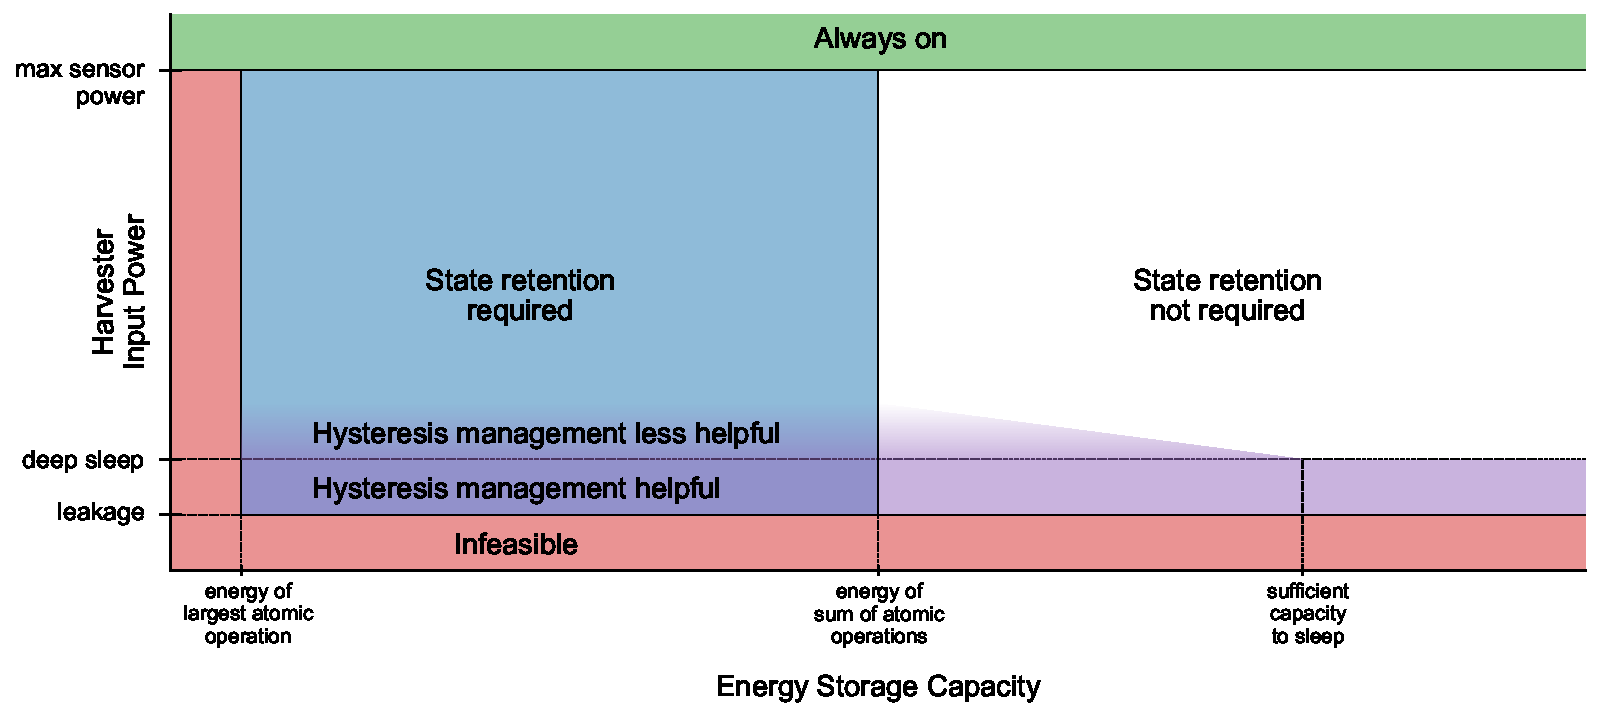
\includegraphics[width=\columnwidth]{figs/chap3/framework/framework}
  \caption{
  %energy-harvesting
  %sensors have different capabilities and requirements
  \normalfont Design space for energy-harvesting sensors based on their energy
  income (assumed constantant for this analysis), energy storage capacity, and workload.
  Workload is represented by the set of atomic operations required by an application, 
  as well as the deep sleep and leakage power.  The plot breaks
  into four regions: \textsf{\color{Green} Always On} 
  or effectively powered, \textsf{\color{BrickRed} Infeasible} due to lack of energy storage or
  leakage higher than harvesting rate, feasible but \textsf{\color{CornflowerBlue} Requires State Retention} 
  to make forward progress, and enough energy storage so that  
  \textsf{State Retention is Not Required}. Additionally, sensors which have high
  power when they enter deep sleep before depleting their
  energy buffer may benefit from \textsf{\color{DarkOrchid} Hysteresis Management} techniques.
  This benefit diminishes with lower sleep currents and higher harvesting potential.
  %With increased capacity, sensors can avoid the complexity of intermittent
  %programming techniques and specialized, reconfigurable power supplies in addition
  %to the other benefits of increased capacity discussed
  %in \cref{sec:store}.
  }
\end{definefigure}


\begin{definefigure}{fig:intuition:eh_worth_it}
  \centering
  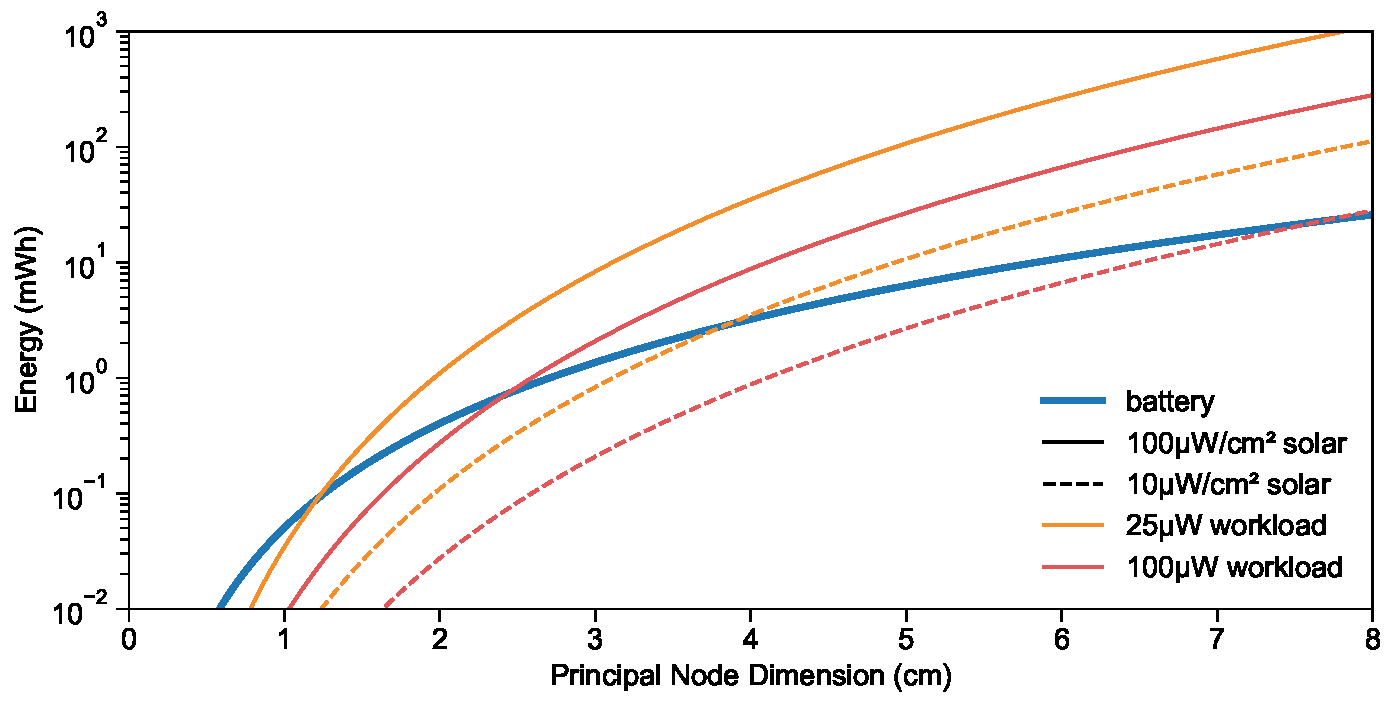
\includegraphics[width=\columnwidth]{figs/is_eh_worth_it_micro.pdf}
  \caption{
  A comparison of preallocated energy and captured energy. Note the logarithmic y-axis scale.
  This figure compares the energy offered by a cubic battery with that of potential harvestable energy captured by a square photovoltaic over the lifetime of the battery. 
  %The lifetime of the battery depends on different workloads, 
  %here represented by the orange (average 25\ssi{\micro\watt}) and red (100\ssi{\micro\watt}) lines. 
  %A solar cell accumulates energy over that same lifetime under different harvesting conditions, represented by a solid line 
  %(100\ssi[per-mode=symbol]{\micro\watt\per\centi\meter\squared}) or dashed line
  %(10\ssi[per-mode=symbol]{\micro\watt\per\centi\meter\squared}).
  %The point at which the harvesting lines (orange, red) cross the battery line (blue) indicate the size at which a similarly sized photovoltaic will harvest the same amount of energy provided by a similar sized battery over its lifetime. 
  At a sufficient size and in sufficient harvesting conditions, while powering an appropriate workload, solar energy-harvesting can provide more energy over the same time frame as a lithium battery.
  }
\end{definefigure}

\begin{definefigure}{fig:intuition:eh_worth_it_nano}
  \centering
  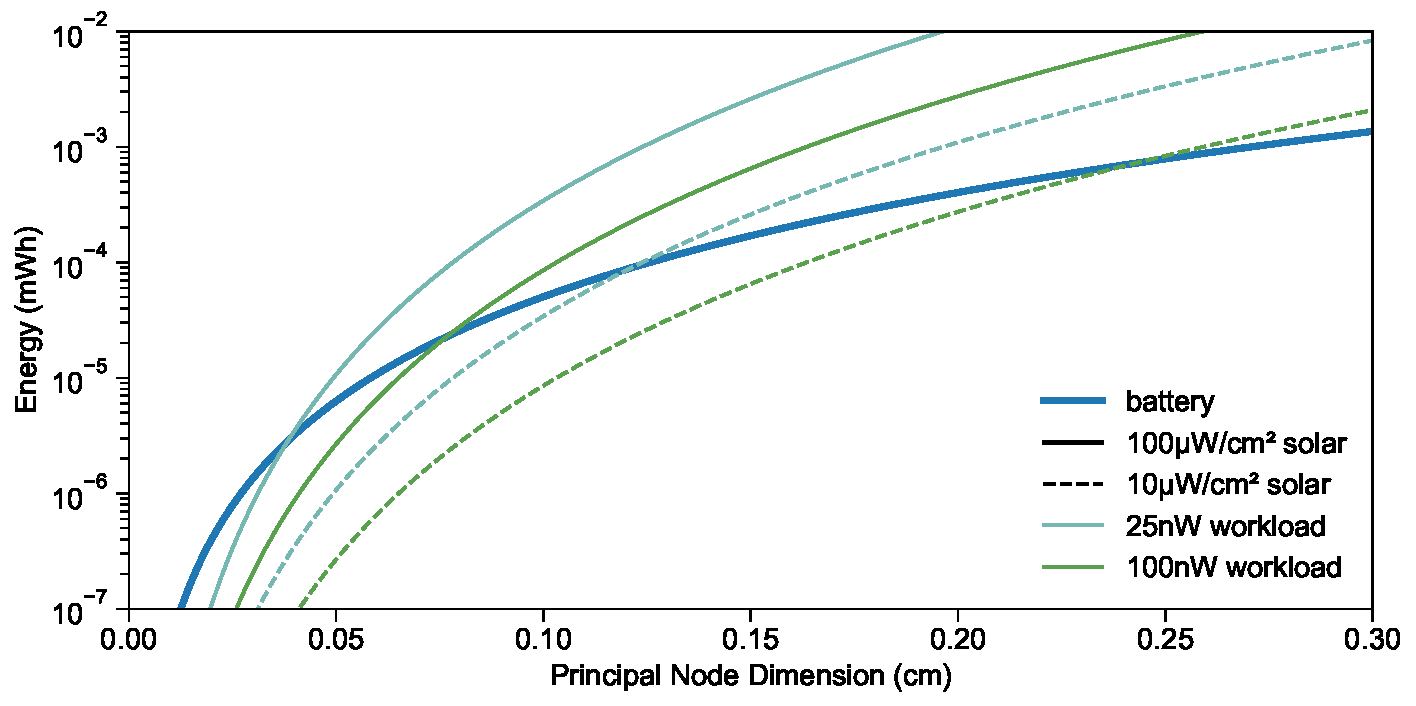
\includegraphics[width=\columnwidth]{figs/is_eh_worth_it_nano.pdf}
  \caption{
  A comparison of preallocated energy and captured energy for \ssi{\nano\watt} applications. 
  This figure is identical to \cref{fig:intuition:eh_worth_it} except that it considers the \ssi{\nano\watt} workloads that characterize millimeter-scale systems.
  A principle node dimension on the order of 1-2\ssi{\milli\meter} is generally sufficient for energy harvesting to collect more energy over a battery, in all but the worst case: a heavier workload with low harvesting potential.
  }
\end{definefigure}


\begin{definefigure}{fig:intuition:compound}
  \centering
  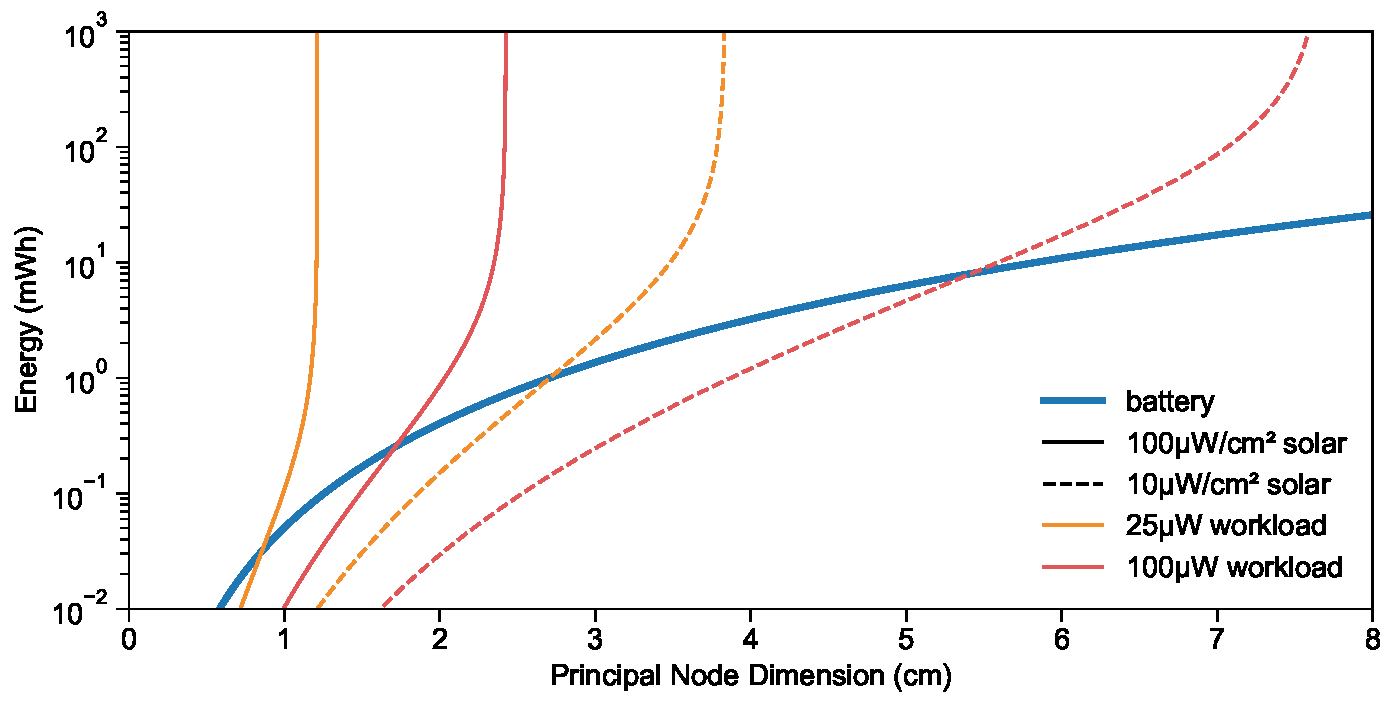
\includegraphics[width=\columnwidth]{figs/is_eh_worth_it_micro_compound.pdf}
  \caption{
    The energy captured by a hybrid system utilizing both harvesting and backup preallocated energy. This figure uses the same scale and line types as \cref{fig:intuition:eh_worth_it}. The addition of energy harvesting to a primary cell system has a compounding effect on lifetime and harvested energy. More harvested energy results in a prolongation of the lifetime of the primary cell. Subsequently, this lifetime extension results in an increase in harvested energy. 
    Because of the increased energy and battery lifetime, the crossing points now shift to the left in the figure, allowing a reduction in volume and area required for a battery and harvester, respectively. 
  }
\end{definefigure}

\begin{definetable*}{tab:intuition:enhants}
            \small
            \begin{tabularx}{\columnwidth}{l | S[table-format=3] | S[table-format=3.1] | S[table-format=4.1] | S[table-format=3.1] }
               % \parbox{1cm}{\raggedleft Irradiance\\Trace} & Total Days & \parbox{1cm}{\centering Average\\Power\\(\textmu W/cm\textsuperscript{2})} & \parbox{1.6cm}{\centering 90\textsuperscript{th} Percentile\\Daily Power (\textmu W/cm\textsuperscript{2})} & \parbox{1.6cm}{\centering 10\textsuperscript{th} Percentile\\Daily Power (\textmu W/cm\textsuperscript{2})} \\\hline
                Irradiance Trace & {Total Days} & {Average Irradiance} & {90\textsuperscript{th} Percentile Daily} & {10\textsuperscript{th} Percentile Daily} \\ 
                \hline
                EnHANTS A   & 393  & 15.1     & 25.0      & 5.2\\
                EnHANTS B   & 375  & 14.9     & 26.0      & 0.80\\
                EnHANTS C   & 310  & 746      & 1610      & 176\\
                EnHANTS D   & 326  & 97.5     & 256.5     & 24.8\\
            \end{tabularx}
            \caption{Summary statistics for the indoor photovoltaic irradiance traces from the EnHANTs dataset~\cite{gorlatova2013networking}.
            Irradiance is expressed in units of \ssi[per-mode=symbol]{\micro\watt\per\centi\meter\squared.}
            }
\end{definetable*}

\begin{definefigure}{fig:intuition:traces}
    \centering
    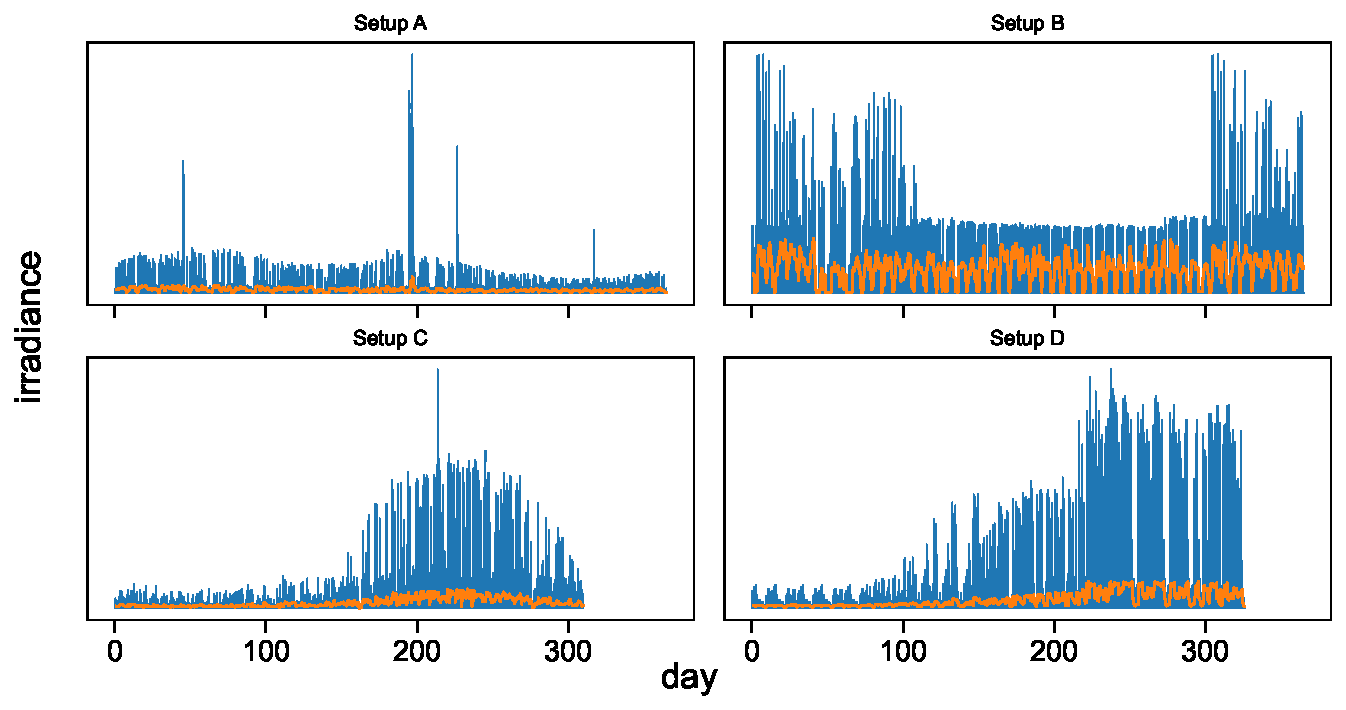
\includegraphics[width=\columnwidth]{figs/chap3/traces/traces.pdf}
    \caption{Each of the four irradiance traces from the EnHANTs dataset represent different lighting and environmental conditions. Here, each trace is min-max normalized to illustrate their individual temporal variance.
    Setup A, B, and D measure irradiance in a student's office. Setup A is located near a south facing window and receives some sunlight. Setup B is located at a bookshelf, and is largely occluded from sunlight. 
    Setup D is located near a west facing window and receives significant sunlight during part of the year. 
    Setup C measures irradiance in a conference room and gets significant sunlight from a north facing window.
    The blue line is the raw irradiance for each trace, while the orange line is a moving average of the irradiance with a day-length window.
    }

\end{definefigure}


\begin{definefigure}{fig:intuition:capacity_sweep}
    \centering
    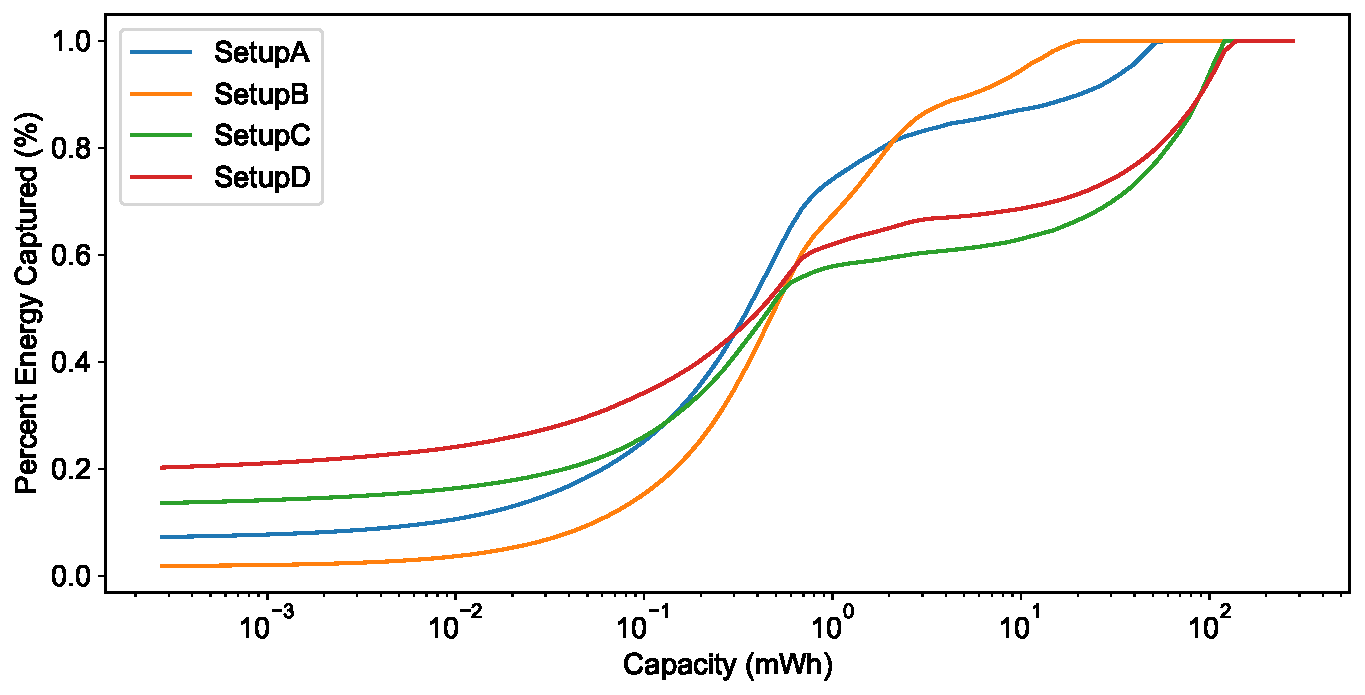
\includegraphics[width=\columnwidth]{figs/chap3/percent_v_capacity_50uW.pdf}
    \caption{
    The percentage of energy captured to satisfy a workload vs a sweep of capacity. 
    This figure assumes a 50\ssi{\micro\watt} average income and workload.
    Note the x-axis log scale.
    Capacity ranges from the order of energy capacity offered by a small 100\ssi{\micro\farad} capacitor, to the capacity offered by a small 100\ssi{\milli\Ah} battery. 
    }
\end{definefigure}

\begin{definefigure}{fig:intuition:required_capacity}
    \centering
    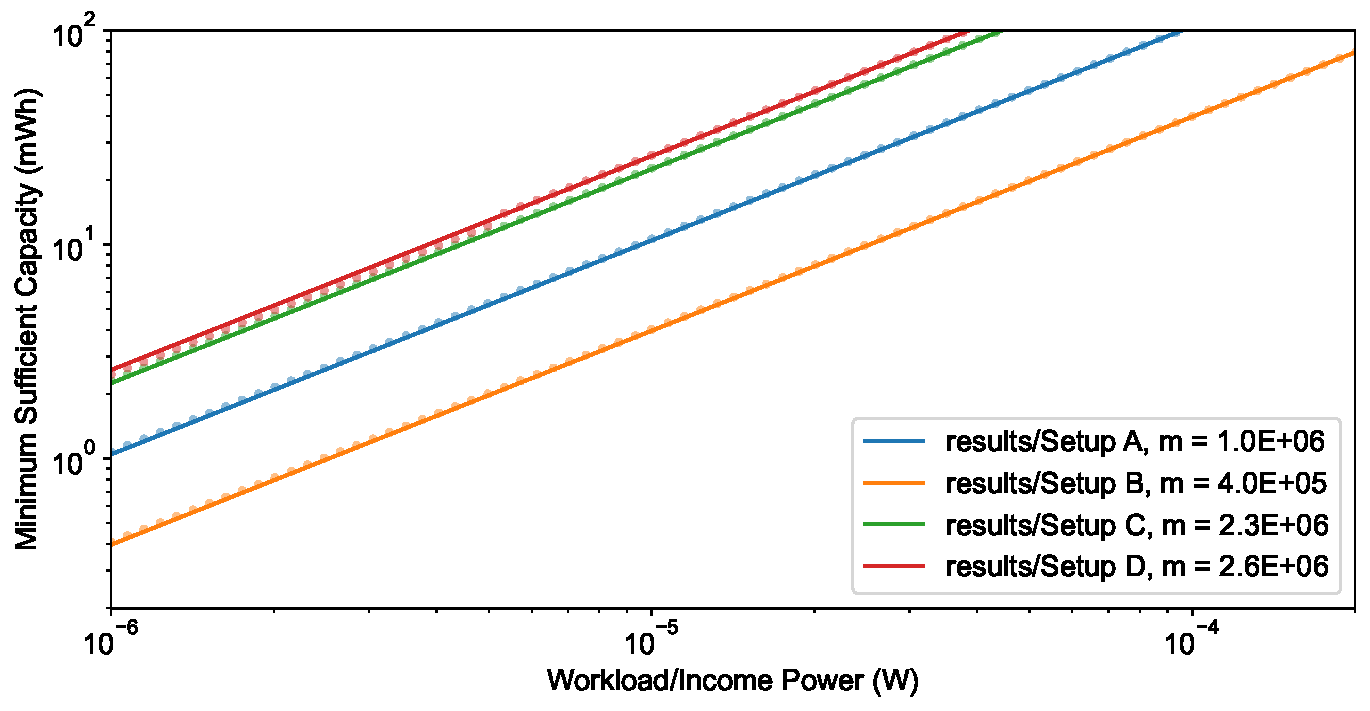
\includegraphics[width=\columnwidth]{figs/chap3/required_capacity.pdf}
    \caption{
    The minimum sufficient capacity to support a workload given an income. Note the x- and y-axis log scale. The average workload and income power are set equal; however the variability of income power is determined by the synthetic EnHANTs traces. The minimum sufficient capacity follows a linear trend with increasing income and workload power. Even though each line appears parallel, lines that are higher up on the y-axis are actually steeper due to the log scale. 
    }
\end{definefigure}